%Classe du Document% 
\documentclass[a4paper,french,12pt]{report}


%Packages utilisés
\usepackage[latin1]{inputenc}
\usepackage[T1]{fontenc}
\usepackage[francais]{babel}
%\usepackage{layout}
%\usepackage{geometry}
\usepackage{setspace}
\usepackage{fixltx2e}
%\usepackage{soul}
%\usepackage{ulem}
%\usepackage{eurosym}
\usepackage{graphicx}
%\usepackage{bookman}
%\usepackage{charter}
%\usepackage{newcent}
%\usepackage{lmodern}
%\usepackage{mathpazo}
%\usepackage{mathptmx}
%\usepackage{url}
%\usepackage{verbatim}
%\usepackage{moreverb}
%\usepackage{listings}
%\usepackage{fancyhdr}
\usepackage{wrapfig}
%\usepackage{color}
%\usepackage{colortbl}
%\usepackage{amsmath}
%\usepackage{amssymb}
%\usepackage{mathrsfs}
%\usepackage{asmthm}
%\usepackage{makeidx}
\usepackage{biblatex}

\bibliography{rapport.bib}

\usepackage[nottoc, notlof, notlot]{tocbibind}


\usepackage{hyperref}
\hypersetup{
	bookmarks=true,
	colorlinks=true,
	linkcolor=black, 
}

\begin{document}

\title{Réalisation d'un panorama}

\author{
	\bsc{Ludovic Lamarche} \\ 
	\bsc{Quentin Perales} \\ 
	\bsc{Elie Poussou} \\ \\ \\ \\
	E.I.S.T.I\\ 
	PAU} 
\date{13 Octobre 2013}


\maketitle
\tableofcontents

%\singlespacing
\onehalfspacing
%\doublespacing 

	\chapter*{Introduction}	
	    Le projet de premier semestre de classe ING1 a pour but d'automatiser la réalisation d'un panorama, c'est-à-dire d'assembler des images qui s'entrecoupent pour réaliser une image générale. Généralement, ce mode de photo est utilisé par les photographes pour obtenir la photo à grande échelle d'un paysage.\\
	    Nous sommes répartis par groupe de 3, Ludovic, Elie et Quentin.\\
	    Pour le premier livrable, nous devons faire un programme en C qui sauvegarde et charge une image pour apprendre les bases du langage, et se familiariser avec le C.\\
	    Ensuite, il faut faire des recherches pour comprendre comment réaliser le panorama, et dégager des méthodes pour parvenir à automatiser sa création.
	\chapter{Avancement du projet}
		    Dans un premier temps, nous avons cherché comment coder en C, faire des recherches plus poussées sur le langage après les cours, comprendre comment les images étaient conçues et apprendre à manipuler les fichiers en général.\\
		    Après quelques essais nous avons conçu la charge et la sauvegarde de l'image avec un tableau d'une seule dimension. Puis, pour faciliter l'utilisation future de l'image, nous avons réalisé une charge et sauvegarde pour une matrice, ce qui permet de visualiser facilement la photo de base.\\
		    Pour tester ces fonctions, nous avons écrit une fonction qui permet de passer d'une image couleur à une image en teinte de gris comme demandée pour le livrable 2.\\
		    Les teintes noires et banches sont données par l'équation suivante : teinteNoire = (teinteR + teinteG + teinteB)/3.
	\section{Ordonnanceur}
	
	\section{Gestion de fichiers}
	\subsection{Enregistrer}
	\subsection{Sauvegarder}
	
	
	\section{Ce qu'il reste à faire}
		    Cependant, tout le code du second livrable ainsi que celui du panorama entier reste à faire même si la réflexion sur le code a été importante au cours de ce premier mois de travail. Plusieurs recherches ont été faites pour comprendre les fonctions à coder pour le livrable 2, notamment la convolution, qui est un produit matriciel entre une matrice de pixels et une matrice en paramètre dans un fichier. Cela fonctionne un peu comme un filtre appliqué à une image. Il suffit ensuite de mettre en place le code dans le programme.\\
	\chapter{Les différentes façons de faire un panorama}
	      Cette seconde partie met en oeuvre les recherches effectuées durant ce premier mois pour savoir comment automatiser un panorama en C. On a dégagé quelques méthodes qui nous semblent possibles pour assembler des images, et donc réaliser le panorama.
		\section{Pré-assemblage}
		    La pré-condition de la fonction Assembler sera de convertir toutes les images en teintes de gris pour éviter de parcourir des tableaux trop importants comme un tableau d'une image couleur (en effet, la largeur de l'image est multipliée par 3). \\
		    Les deux premières méthodes ont été plus ou moins mises en place par nous, ces méthodes sont lourdes pour l'ordinateur. \\
		    La dernière méthode est une synthèse des recherches, cette méthode revient souvent mais n'est pas clairement expliquée. Le but est de récupérer un ensemble de points appelés "coins" de l'image. Le point obscur de cette méthode est donc de savoir comment les repérer dans les deux images pour les assembler.\\
		    Pour assembler les images, on n'en considère que deux à la fois.
		\section{Première méthode : Point par point}
		    %Quentin
		    Cette méthode est la plus précise et la plus simple à comprendre. On cherche à faire correspondre chaque pixel d'une image, à une autre image.
		    On prend un pixel dans la première image et on cherche un pixel d'une même teinte dans l'autre image. Ce qui veut dire que l'autre image va être parcourue en entier pour trouver une correspondance. Si une correspondance est trouvée, on cherche à agrandir cette correspondance en faisant correspondre une matrice de pixels. Plus elle va être grande, plus l'assemblage entre les images est probable. Si une matrice sur le bord d'une image correspond à une matrice sur le bord d'une autre image, on les assemble en enregistrant les décalages en hauteur et largeur. Ce code est très coûteux pour la machine, surtout si la taille des images est importante. Il faudra alors manipuler des matrices de plus d'un million d'entiers chacune.
		    
		    \begin{figure}[h]
		     \begin{center}
		      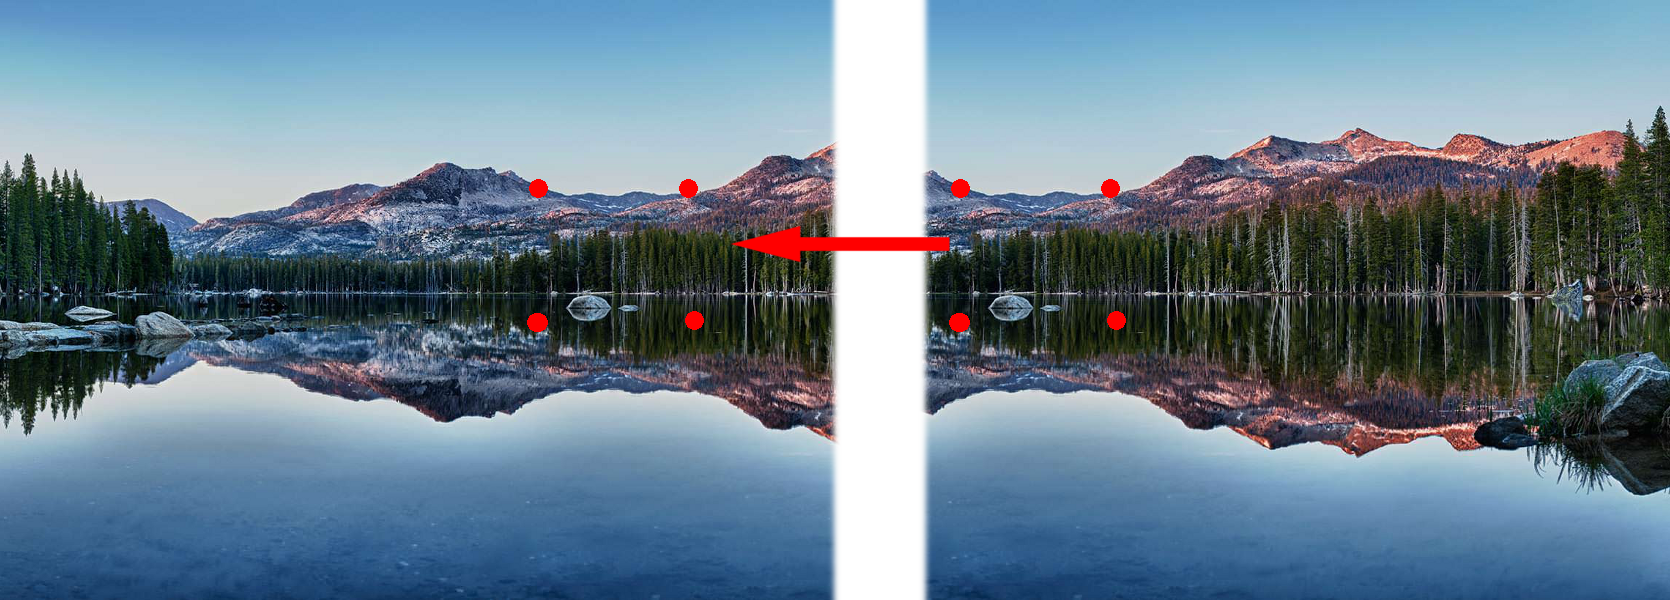
\includegraphics[scale=.23]{images/panorama3.png}
		      \caption{Schéma de la méthode point par point}
		     \end{center}
  
		    \end{figure}
		\section{Seconde méthode : Les lignes ou colonnes}
		    %Elie
		    Pour cette deuxième méthode, on prend les lignes et les colonnes de pixels qui se situent sur les bords des deux images que l'on souhaite assembler. \\
		    Pour chaque ligne et colonne, on prend aléatoirement un certain pourcentage de pixels (25\% par exemple), et on cherche des correspondances entre les deux images grâce à ces points.\\
		    Si l'on trouve des correspondances, on peut étendre la comparaison aux lignes ou colonnes voisines pour pouvoir vérifier, plus il y aura de points en commun, plus l'assemblage sera précis.\\
		    Si la correspondance est validée, on peut assembler les deux images à l'endroit où l'on a trouvé des pixels communs.\\
		    Il faudra ensuite gérer le décalage qui fait apparaître des zones noires.\\
		   Cette seconde méthode est moins gourmande que la précédente car on se concentrera sur les lignes et colonnes qui se situent sur le bord de l'image.
		    
		    \begin{figure}[h]
		     \begin{center}
		      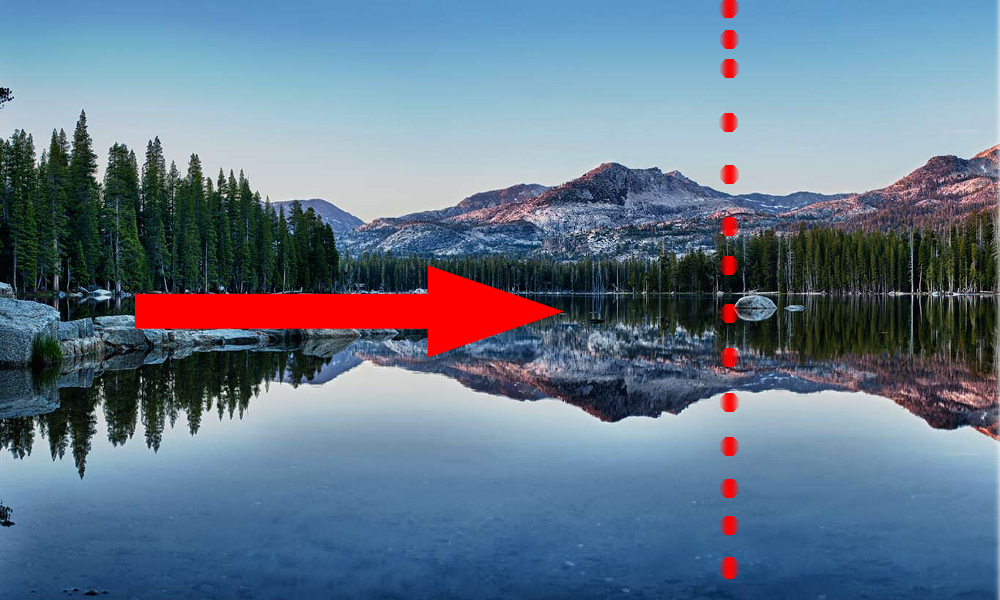
\includegraphics[scale=.18]{images/panorama2.png} 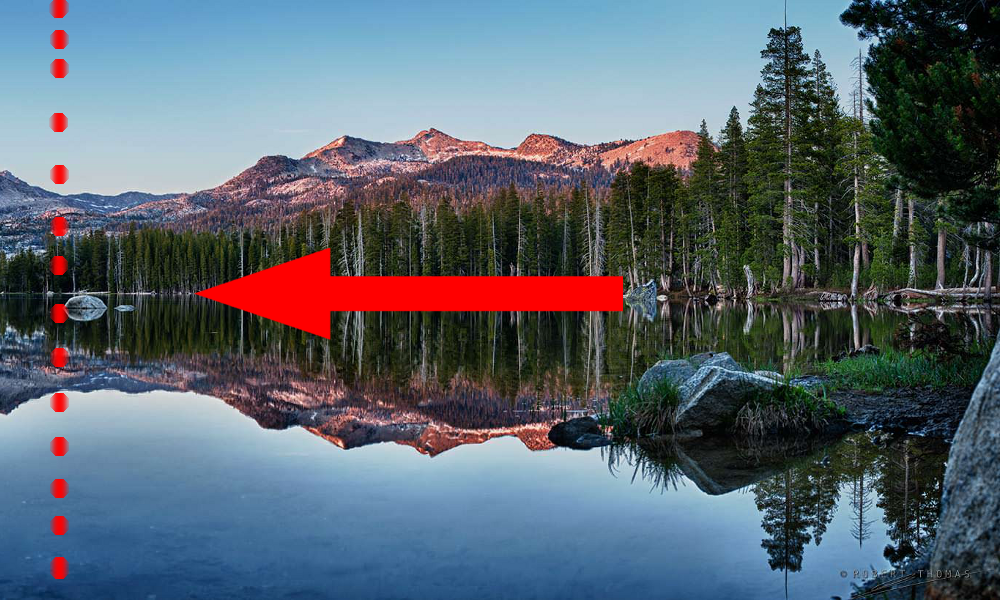
\includegraphics[scale=.18]{images/panorama1.png}
		      \caption{Schéma de la méthode des lignes ou des colonnes}
		     \end{center}
  
		    \end{figure}
		    
		\section{Troisième méthode : Méthode des coins}
		    %Quentin
		    Dans un premier temps, il faut repérer les "coins" de l'image. Une des possibilités peut être l'utilisation de l'algorithme Features from Accelerated Segment Test (FAST). Pour cela, il faut définir un seuil inférieur et un seuil supérieur. Ensuite, on définit le rayon d'un cercle qui sera constant. On choisit ensuite un pixel quelconque et on repère les pixels sur le contour du cercle de ce pixel. Voici un schéma de la situation autour d'un pixel.\\
		    
		    

		    \begin{figure}[h]
		     \begin{center}
		      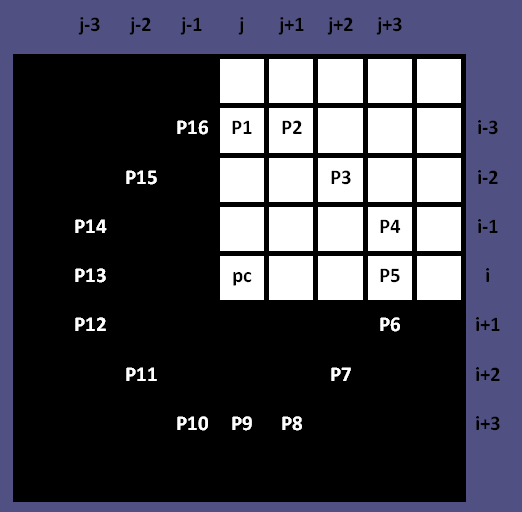
\includegraphics[scale=.25]{images/panorama4.png}
		      \caption{Schéma du panorama avec la méthode des coins\cite{operationpixel}}
		     \end{center}
  
		    \end{figure}	    
		    
		    
		    Ainsi, on reçoit un tableau de valeurs, ici 16, d'echelle de gris. On transforme ensuite le tableau de la manière suivante :
		    \begin{itemize}
		     \item si la valeur est inférieure à la valeur de seuil inférieur, on mets -1 dans le tableau ;
		     \item si la valeur est enre les deux valeurs de seuil, on lui assigne 0 ;
		     \item si la valeur est supérieure à la valeur de seuil supérieure, on lui assigne 1.
		    \end{itemize}
		    En choisissant plusieurs points de la sorte, on cherche alors dans l'autre image une corres entre certains pixels. Si il y a plusieurs identifications, on assemble les deux images de manière à ce qu'elles coïncident.
		\section{Post-assemblage}
		    En fin d'assemblage, on obtient deux images accolées. Pour remplir le reste de l'image résultat, on y met des pixels gris. On considère ce résultat comme une image sourcee pour réutiliser l'algorithme d'assemblage de deux images si il reste des images non utilisée pour réaliser le panorama. Si aucune correspon n'est trouvée entre les deux images, on les conserve et on utilise les autres images pour essayer de reconstituer une image susceptible de trouver des correspondances avec les images non-utilisées.
	\chapter*{Conclusion}
	    %Aucune idée
	    Pour conclure, nous pensons que ce projet nécessite autant d'heures de codage que d'heures de réflexion sur la façon de créer notre programme, et surtout pour comprendre comment automatiser un panorama. Pour ce second livrable, nous avons pour but de faire les fonctions demandées assez rapidement pour ensuite nous avancer sur le dernier livrable, ce qui nous permettra de réfléchir plus profondément sur les erreurs que nous allons rencontrer.
	    \cite{operationpixel}
	    \newpage
	    
\printbibliography
\end{document}
